\subsection{Experiments}
\subsubsection{Experiment 1}
The first experiment performed compares the different architectures using the 
\emph{Mean Squared Error (MSE)} loss 
function.
The baseline model is able to reach the goal, but with little precision and 
often colliding with the object, as shown 
in Figure \ref{fig:baseline}.

\begin{figure}[htbp]
	\centerline{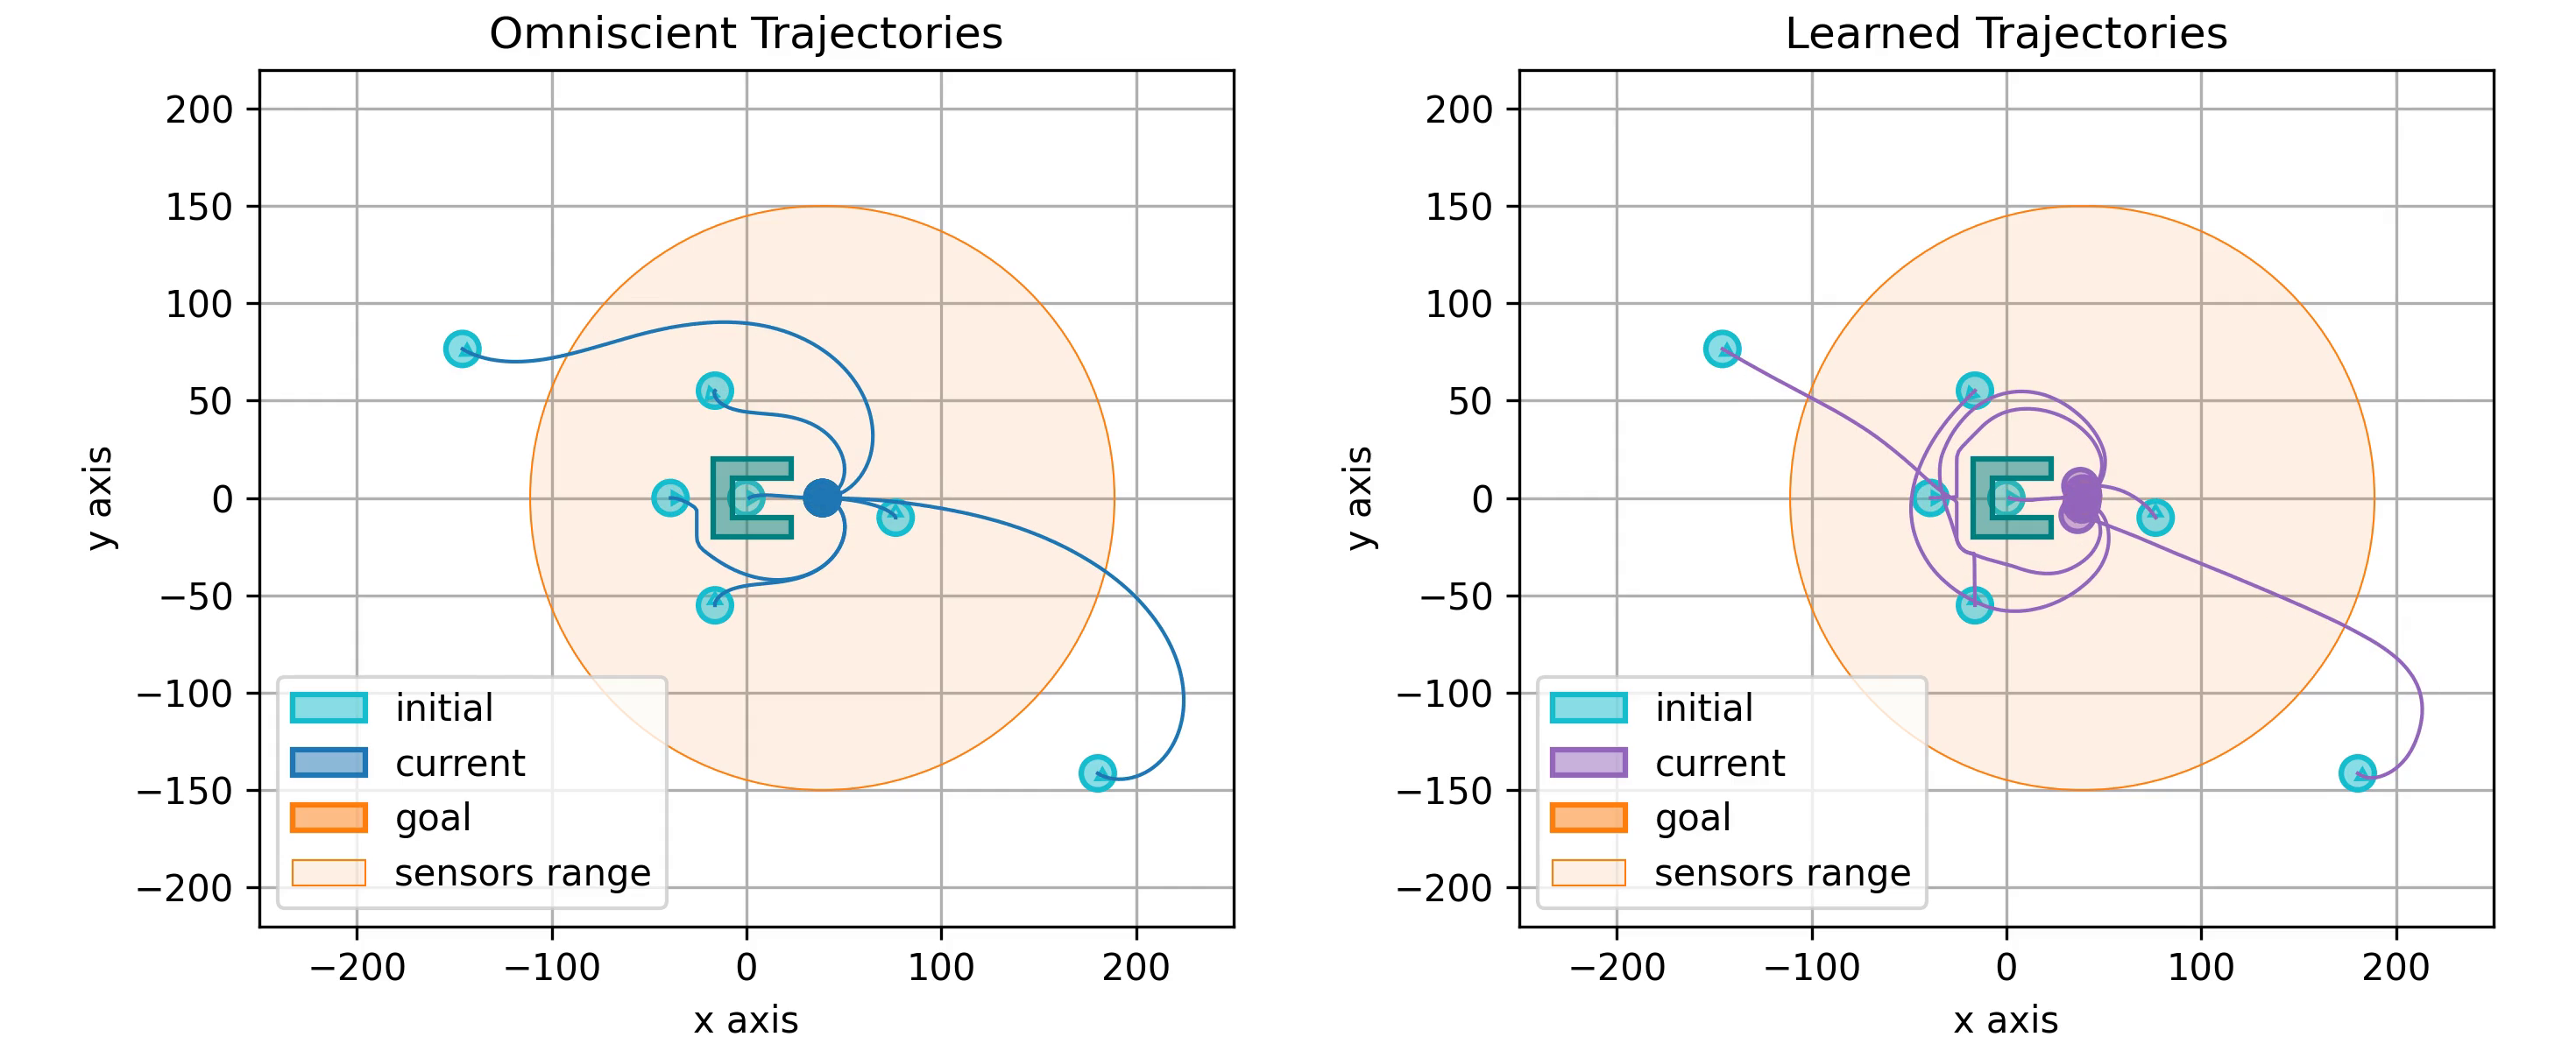
\includegraphics[width=\columnwidth]{experiments/1/demo-trajectories-baseline}}
	\caption{Trajectories of the controller learned from the baseline network.}
	\label{fig:baseline}
\end{figure}

\begin{figure}[htbp]
	\centerline{\includegraphics[width=\columnwidth]{experiments/1/regression-validation-baseline}}
	\caption{$R^2$ regressor on the validation set of the baseline network.}
	\label{fig:regression-baseline}
\end{figure}


Adding either max pooling or dropout alone does not solve the problem, but 
combining them results in a visible 
improvement: the robot reaches the goal position more precisely even if 
oscillating a bit.

\begin{figure}[htbp]
	\centerline{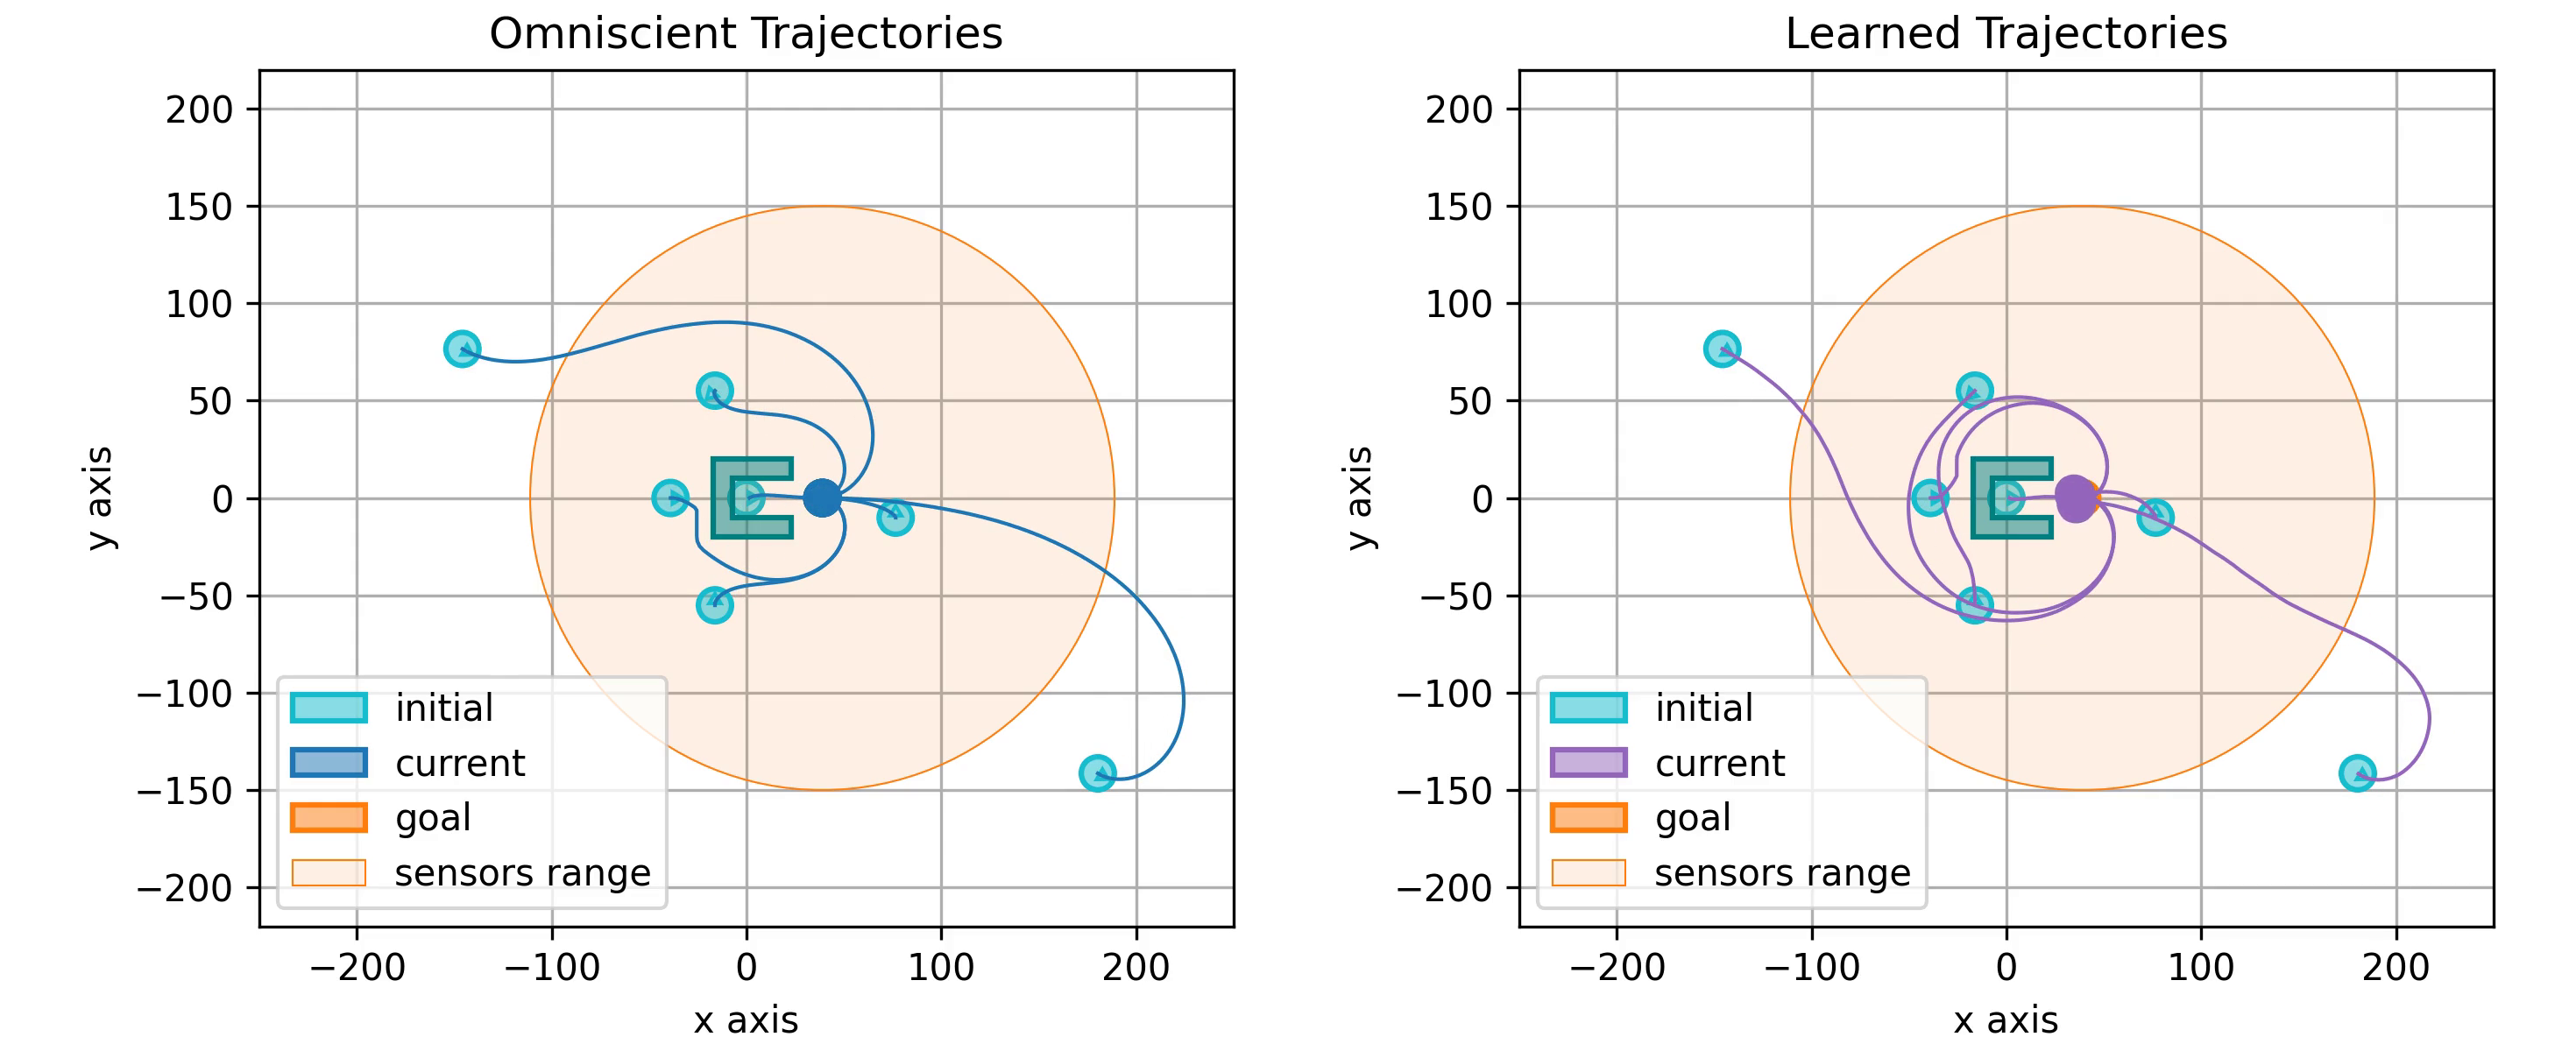
\includegraphics[width=\columnwidth]{experiments/1/demo-trajectories-maxpool+dropout}}
	\caption{Trajectories of the controller learned from the max pooling + 
	dropout network.}
	\label{fig:maxpool+dropout}
\end{figure}

\begin{figure}[htbp]
	\centerline{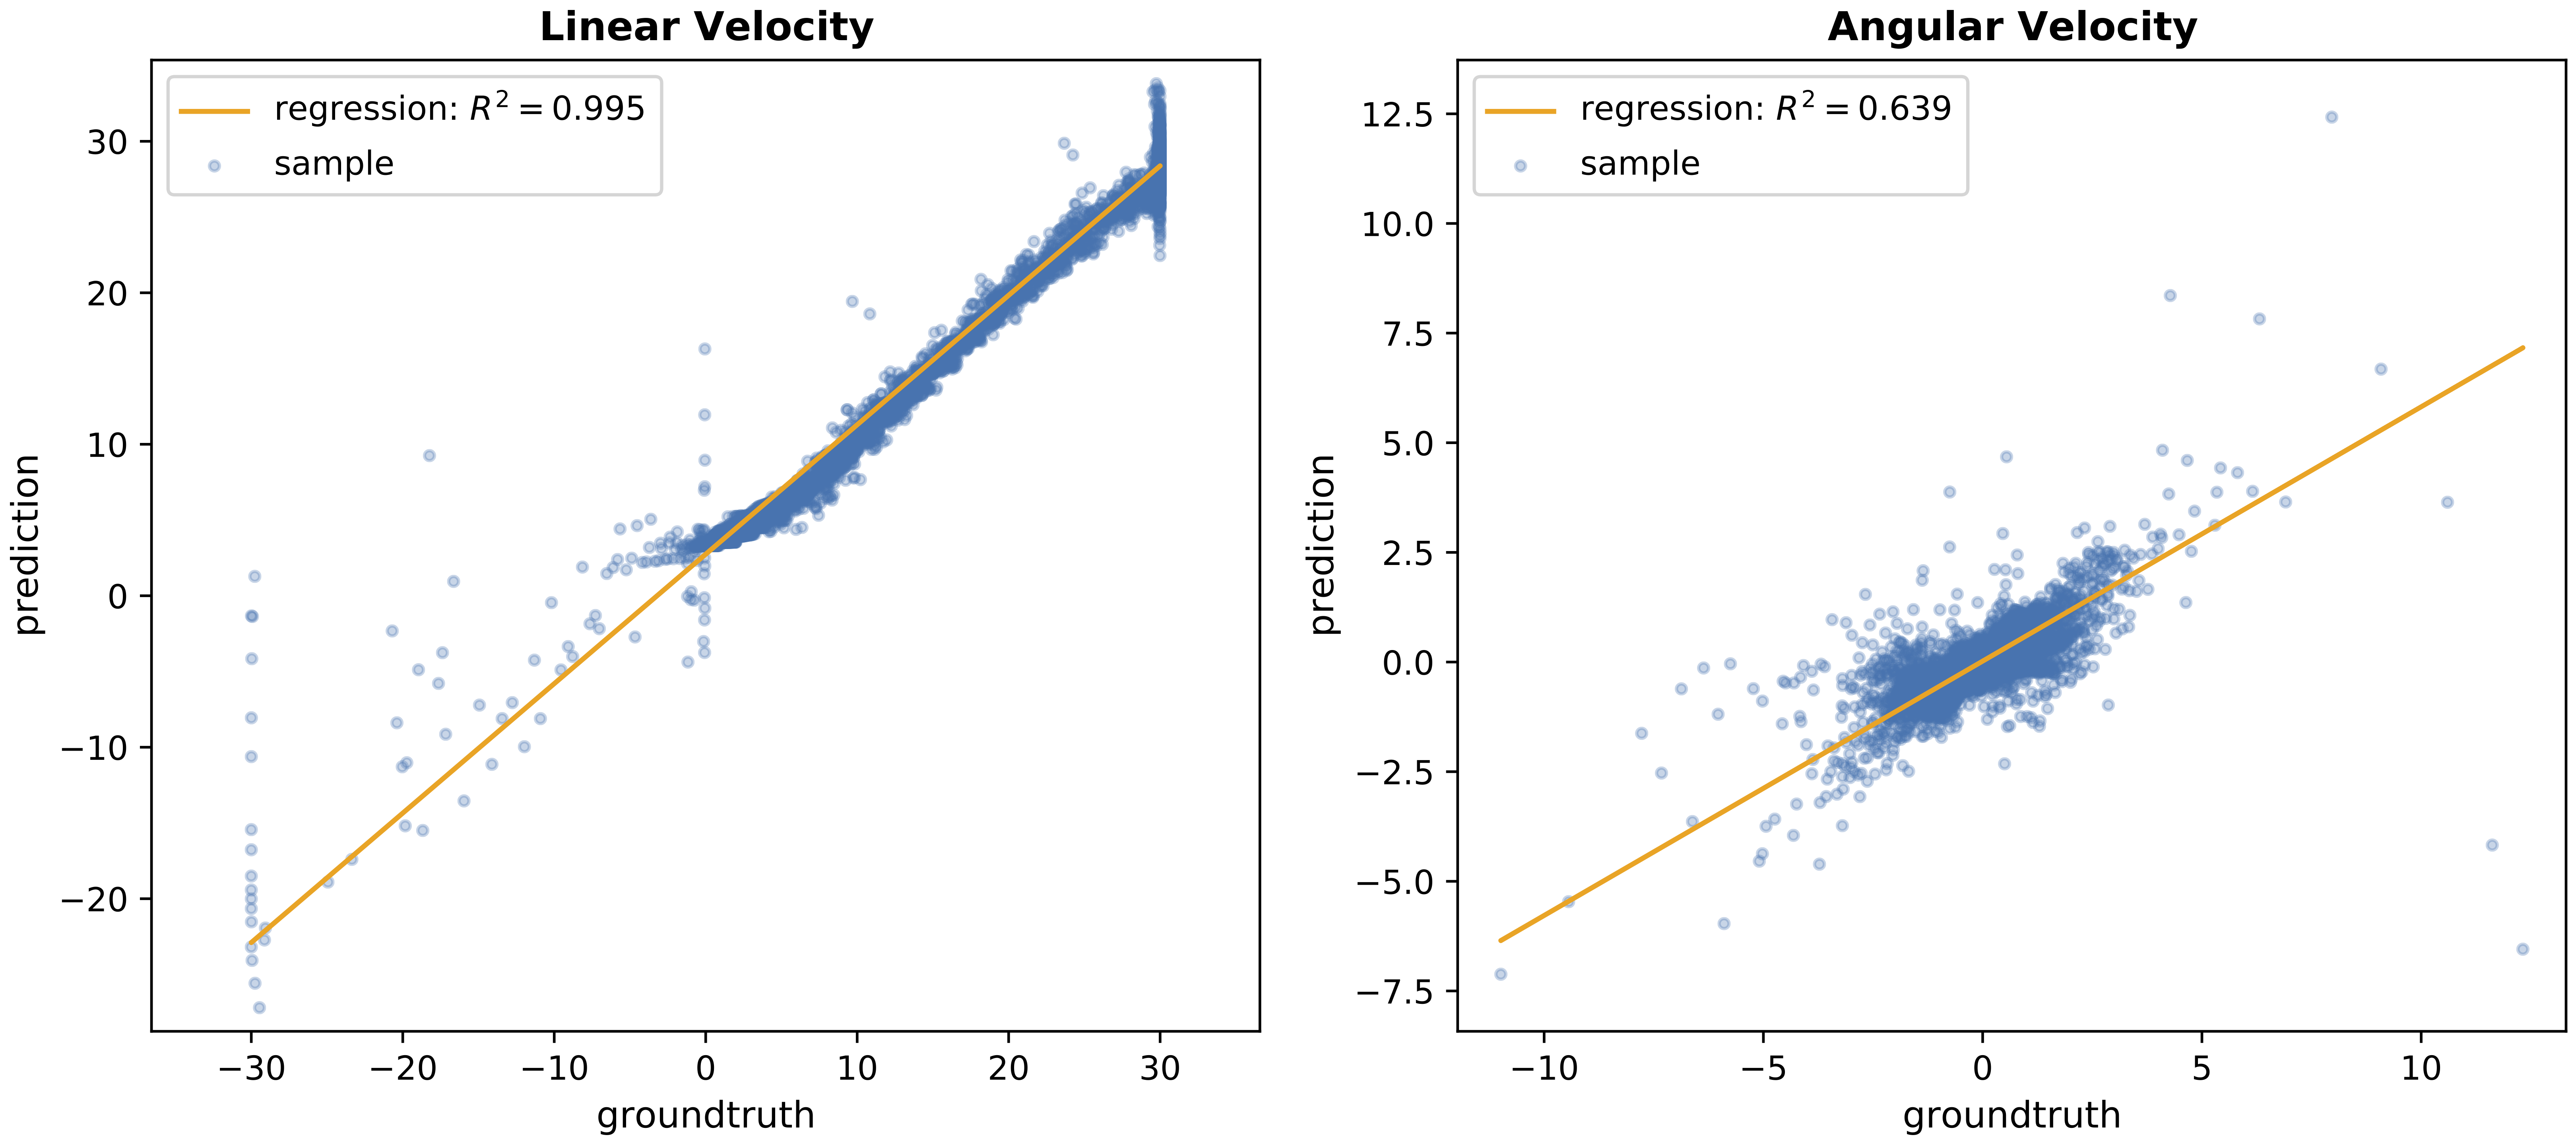
\includegraphics[width=\columnwidth]{experiments/1/regression-validation-maxpool+dropout}}
	\caption{$R^2$ regressor on the validation set of the max pooling + dropout 
	network.}
	\label{fig:regression-maxpool+dropout}
\end{figure}

The regression coefficients of the angular velocity, displayed in Figure 
\ref{fig:regression-baseline} and \ref{fig:regression-maxpool+dropout}, 
increase from $0.54$ to $0.64$, confirming the improvement of the second model.
A shown in Figure \ref{fig:loss}, it shows also a lower validation loss (in 
red) and does not overfit toward the end of training, like the baseline model 
(in orange).

\begin{figure}[htbp]
	
\centerline{\includegraphics[width=.8\columnwidth]{experiments/1/loss}}
	\caption{Comparison of the losses among train and validation sets.}
	\label{fig:loss}
\end{figure}

Finally, the end positions are more tightly clustered over the goal.
Both the heatmaps in Figure \ref{fig:heatmaps} show a tendency to rotate around 
the object, which are caused by its symmetry. We will explore this in the third 
experiment \ref{fig:final-positions}.

\begin{figure}[htbp]
	\centerline{\includegraphics[width=\columnwidth]{experiments/1/heatmaps}}
	\caption{Positions heatmaps.}
	\label{fig:heatmaps}
\end{figure}

\begin{figure}[htbp]
	\centerline{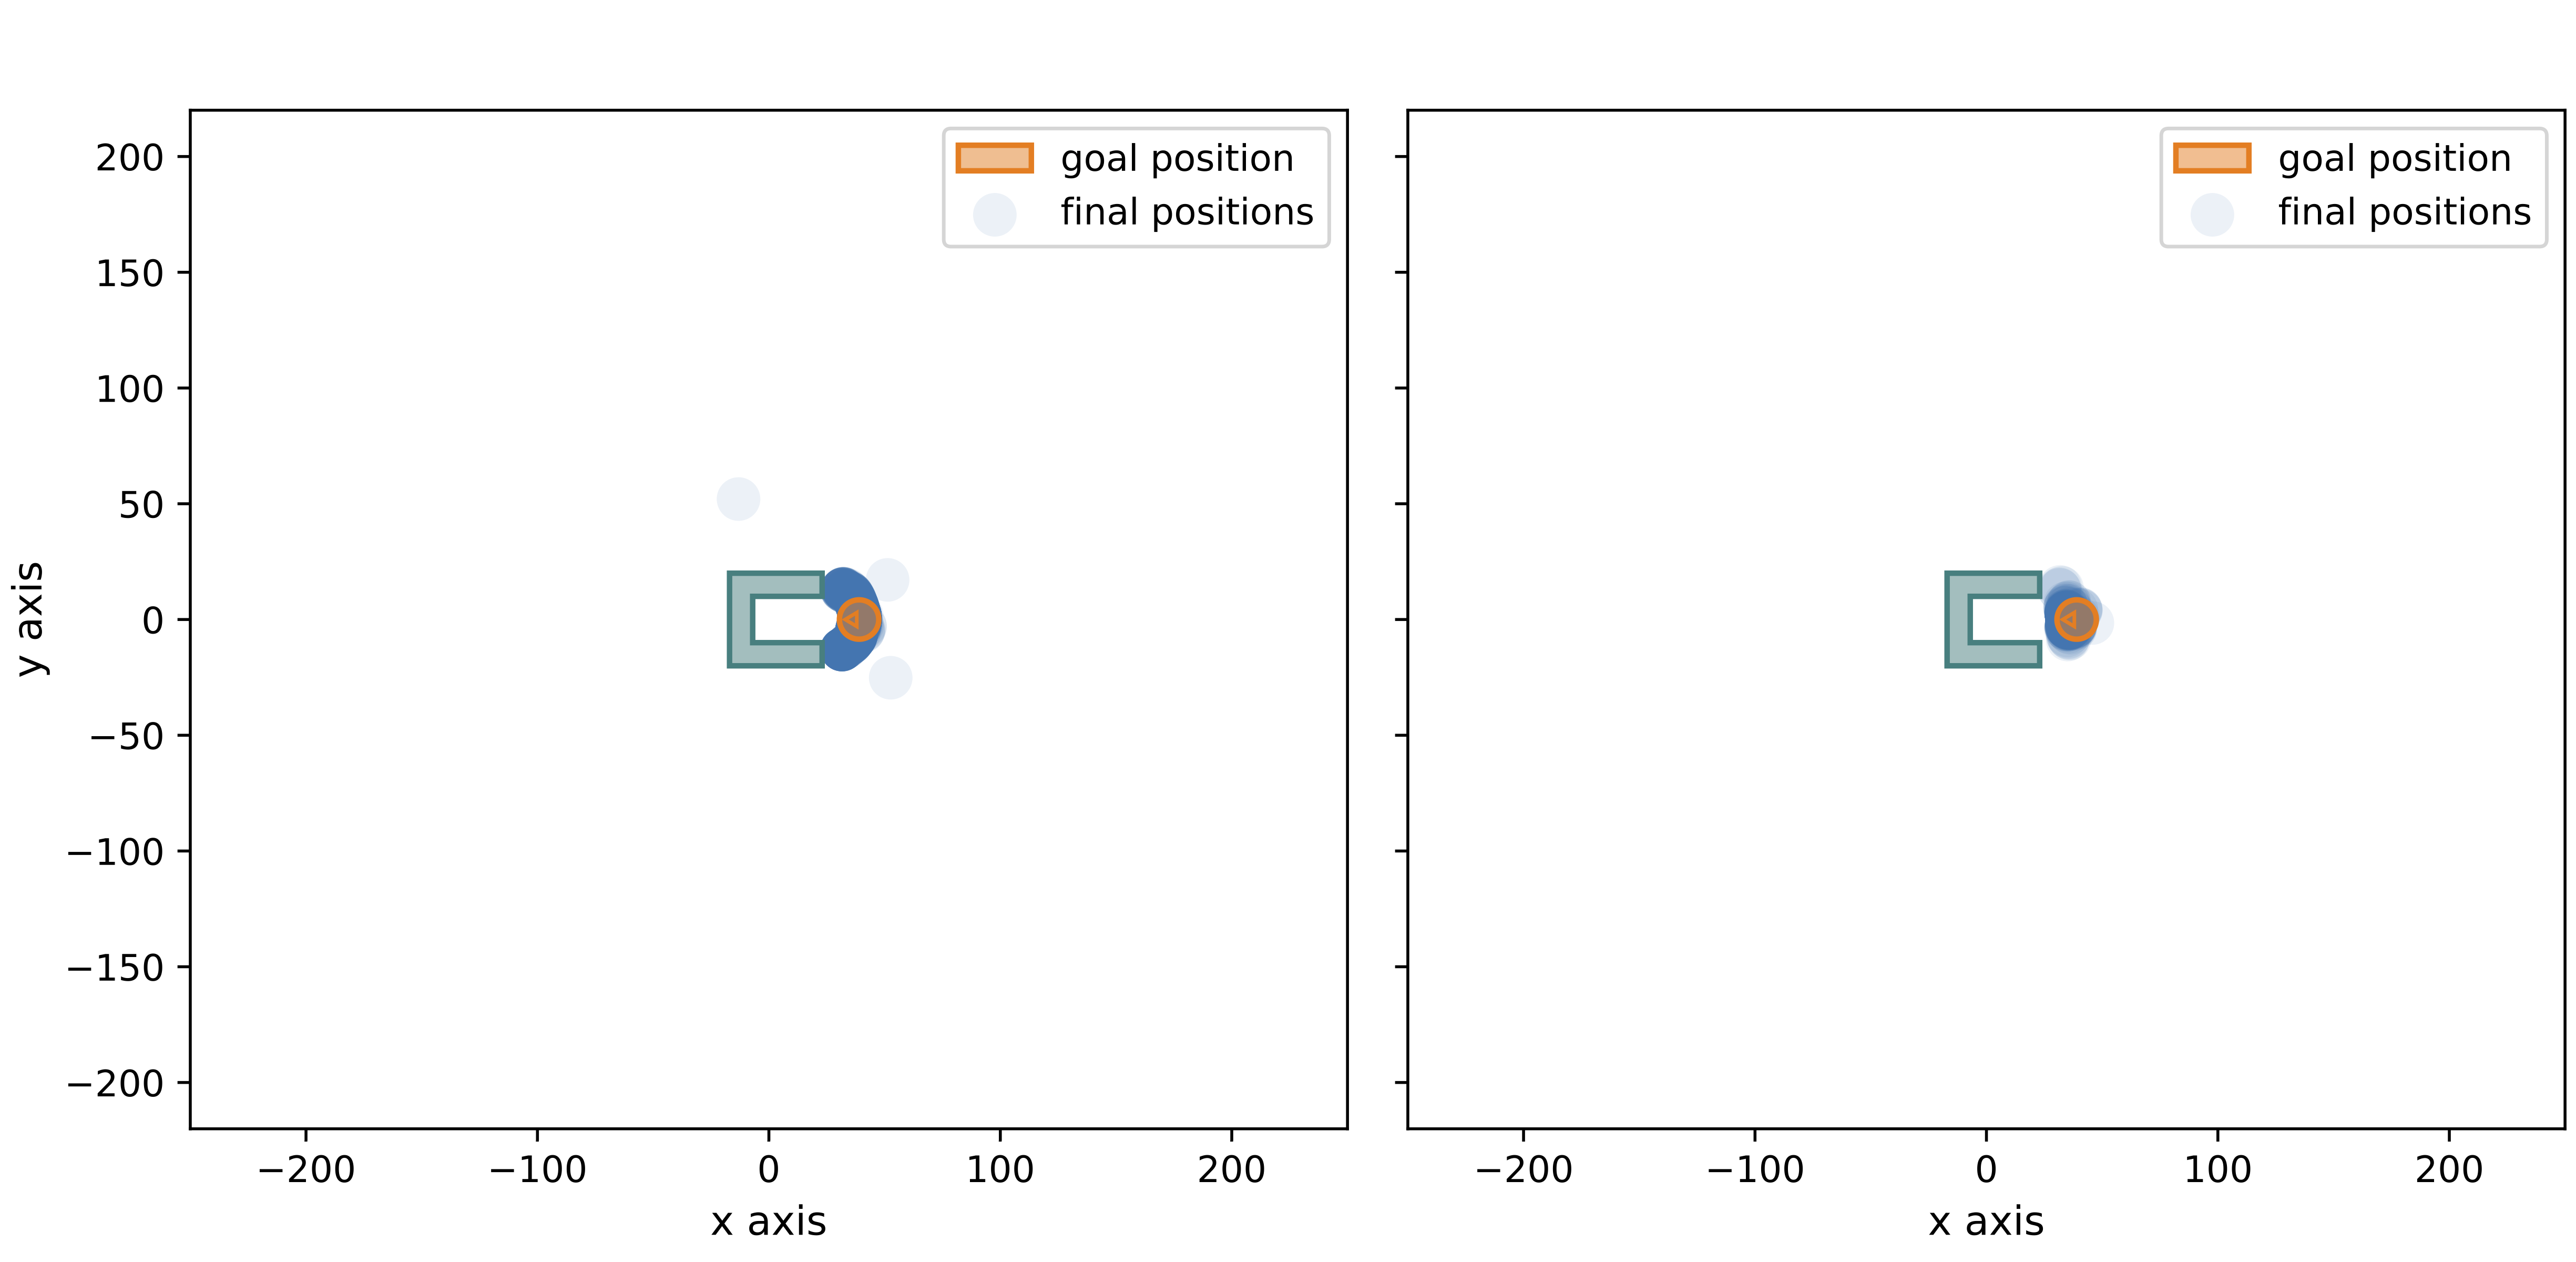
\includegraphics[width=\columnwidth]{experiments/1/final-positions}}
	\caption{Final positions.}
	\label{fig:final-positions}
\end{figure}


Even though the overall behaviour of this model is good, the main drawback is a 
slight systematic error in the final orientation that we can see in Figure 
\ref{distance-from-goal-learned}.

\begin{figure}[htbp]
	\centerline{\includegraphics[width=\columnwidth]{experiments/1/distances-from-goal}}
	\caption{Distance from goal over time.}
	\label{fig:distance-from-goal-learned}
\end{figure}

\subsubsection{Experiment 2}
The second experiment performed compares the previous model with one with the 
same network architecture, but that uses a second loss function, \emph{Smooth 
L1} \cite{smoothl1}, which is less sensitive to outliers than \emph{MSE} and in 
some cases prevents exploding gradients. It is computed using \eqref{smoothl1}

\begin{equation}
\text{loss}(x, y) = \frac{1}{n}\sum_{i}z_i
\label{smoothl1}
\end{equation}

where $z_i$ is given by

\begin{equation}
z_i = 
\begin{cases}
0.5 (x_i-y_i)^2, &\text{ if } |x_i-y_i|<1 \\
|x_i-y_i| - 0.5, &\text{ otherwise}
\end{cases}
\end{equation}

 
Although it results in less precise final positions, it solves the oscillation 
issue, as shown in Figure \ref{fig:demo-trajectories}.

\begin{figure}[htbp]
	\centerline{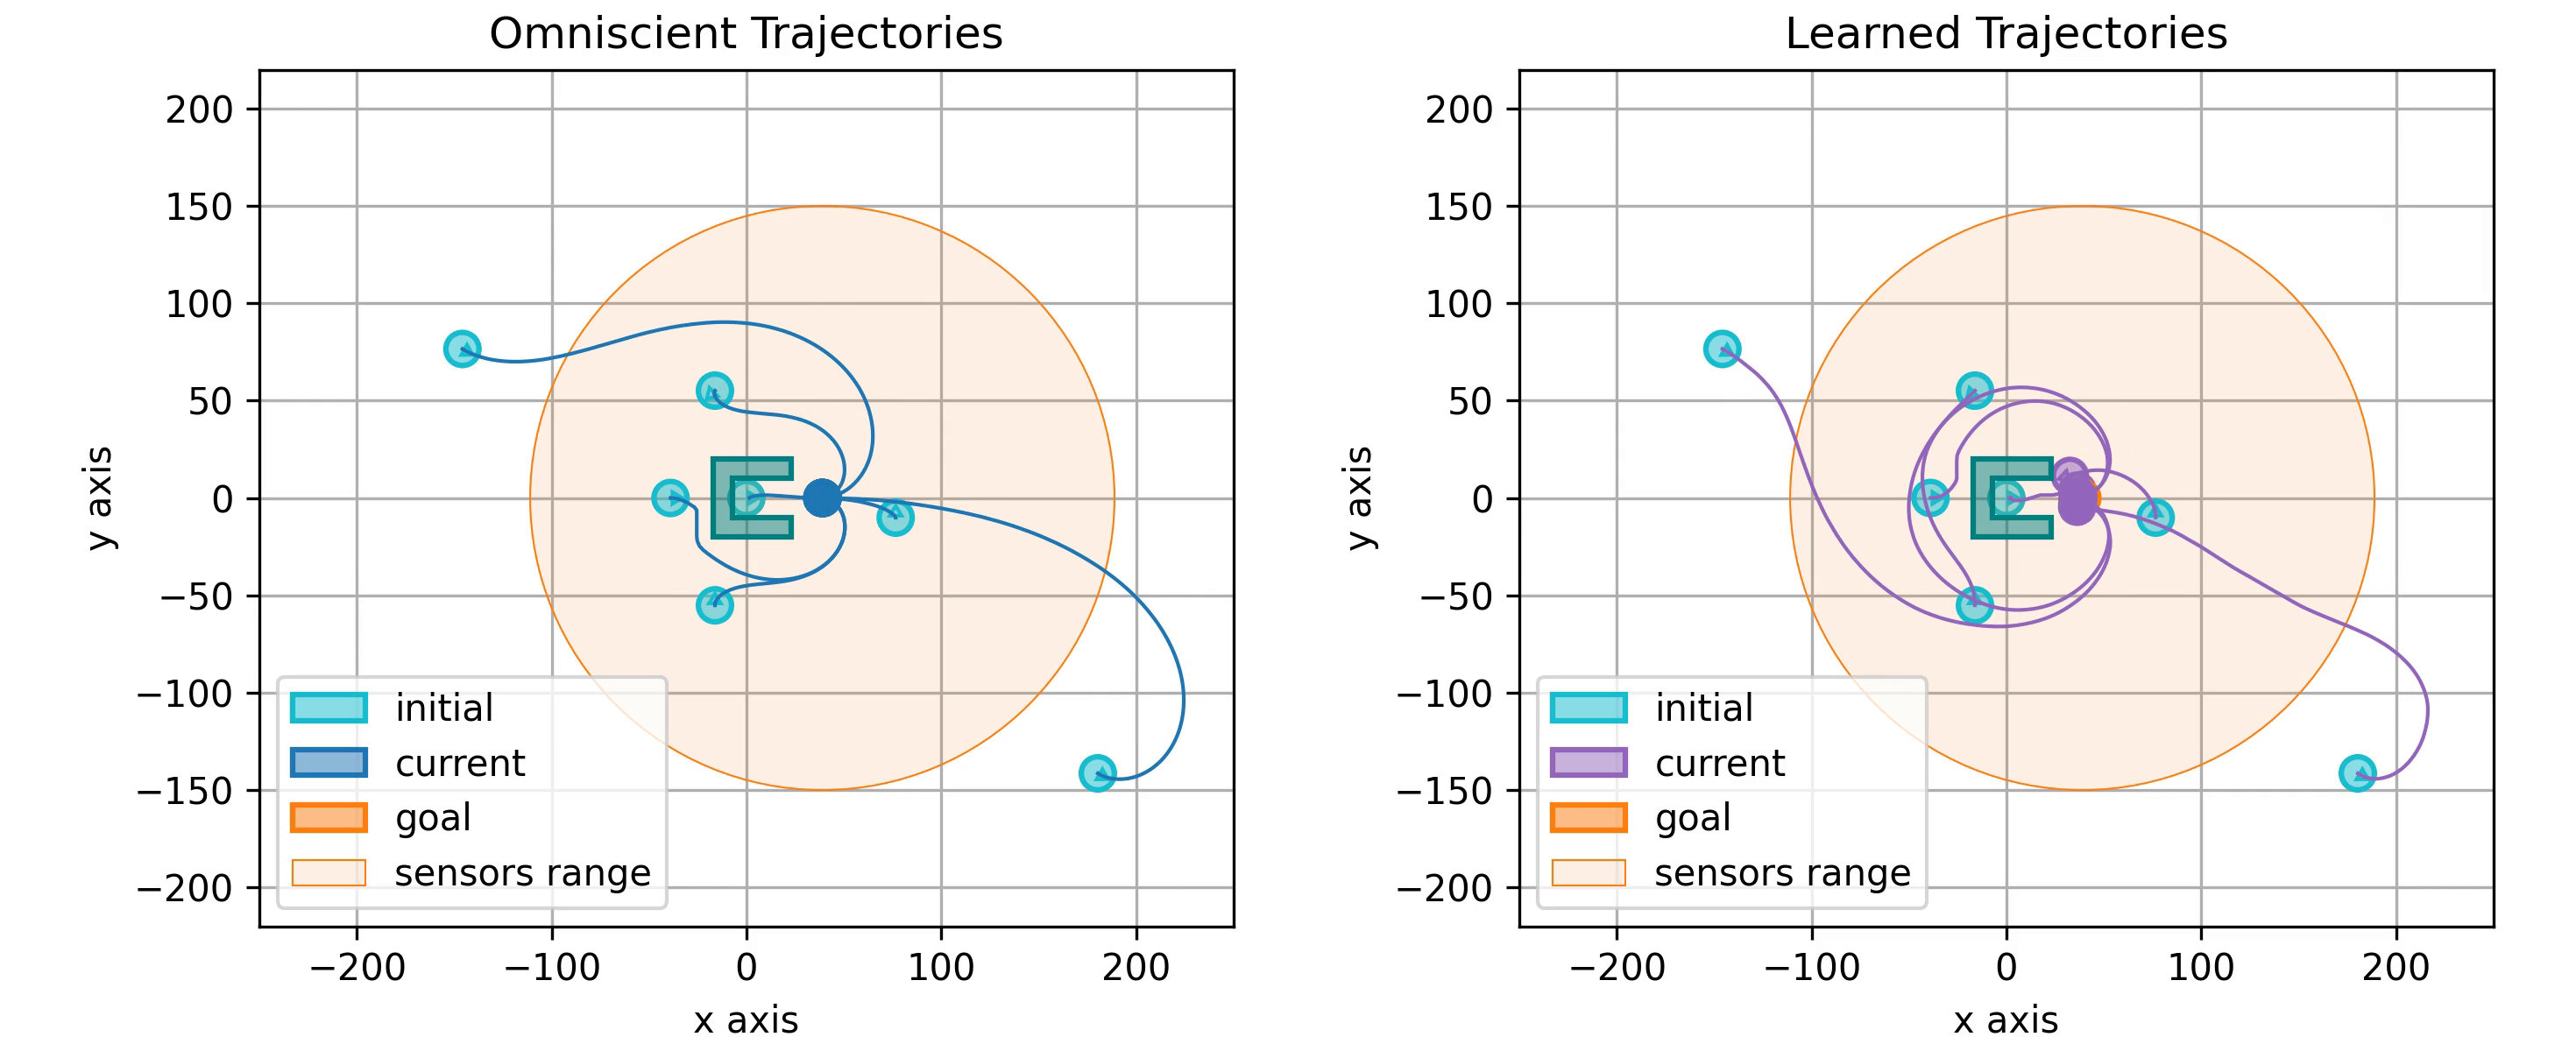
\includegraphics[width=\columnwidth]{experiments/2/demo-trajectories}}
	\caption{Trajectories.}
	\label{fig:demo-trajectories}
\end{figure}

The regression coefficients of the angular velocity, shown in Figure 
\ref{fig:regression-validation}, decrease from $0.64$ to $0.58$, confirming the 
superiority of the previous model.

\begin{figure}[htbp]
	\centerline{\includegraphics[width=\columnwidth]{experiments/2/regression-validation}}
	\caption{$R^2$ regressor on the validation set.}
	\label{fig:regression-validation}
\end{figure}

\subsubsection{Experiment 3}

The monochromatic goal object shown so far has symmetries that make the 
trajectory to follow ambiguous, causing the robots converge to the goal in a 
spiral path, as visualised in Figure \ref{fig:demo-circle-trajectories}.
This issue is solved in this final experiments that consists in removing any 
ambiguity in the sensor readings by using a polychromatic goal object that has 
different colours for each of its faces.

\begin{figure}[htbp]
	\centerline{\includegraphics[width=\columnwidth]{experiments/3/monochromatic-polychromatic}}
	\caption{Comparison of the trajectories of the monochromatic and 
	polychromatic goal object.}
	\label{fig:demo-circle-trajectories}
\end{figure}

The same network architecture and loss function of the first experiment are 
used to train the the model with a polychromatic object, and result in a 
significant improvement both in regression coefficient of the angular 
velocities, shown in Figure \ref{fig:regression-3}, and in training and 
validation losses (in green and red), in Figure \ref{fig:loss-3}.

\begin{figure}[htbp]
	\centerline{\includegraphics[width=\columnwidth]{experiments/3/regression-validation}}
	\caption{$R^2$ regressor on the validation set.}
	\label{fig:regression-3}
\end{figure}

\begin{figure}[htbp]
	
	\centerline{\includegraphics[width=.8\columnwidth]{experiments/3/loss}}
	\caption{Comparison of the losses among train and validation sets.}
	\label{fig:loss-3}
\end{figure}

Finally, Figure \ref{fig:heatmap-final-positions} shows how the end positions 
are more tightly clustered over the goal than before. Moreover, the model is 
able to follow the optimal trajectories without rotating around the object.
Also in terms of convergence, the robot reaches the goal more precisely, as 
shown in Figure \ref{fig:distance-from-goal-learned3}, and sometimes even 
faster than the omniscient controller.

\begin{figure}[htbp]
	\centerline{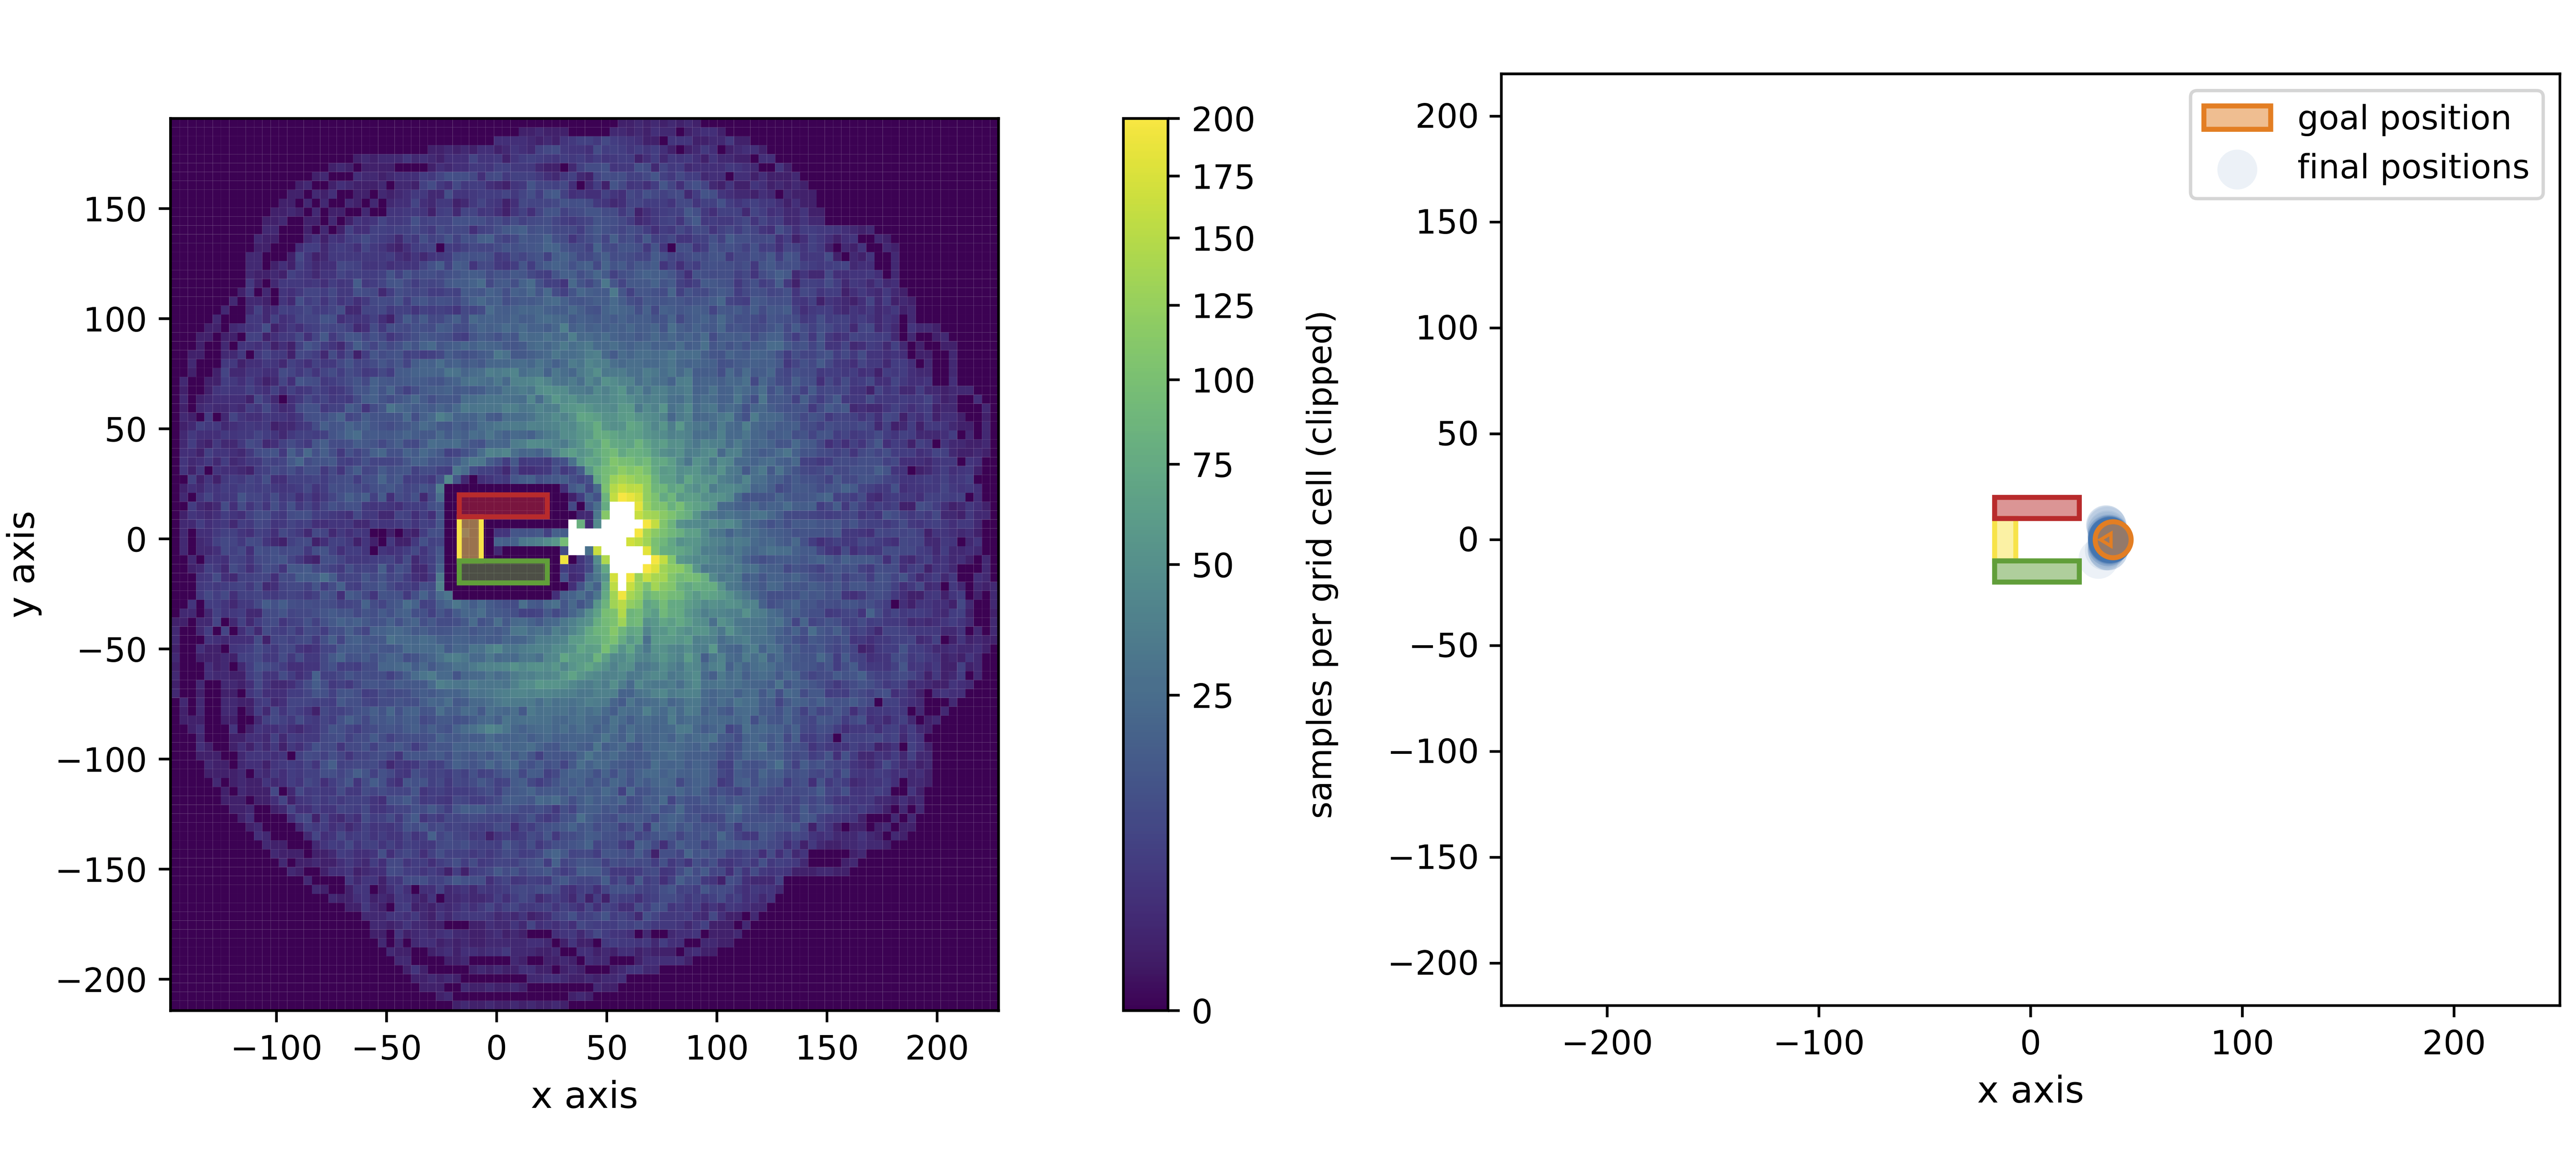
\includegraphics[width=\columnwidth]{experiments/3/heatmap-final-positions}}
	\caption{Positions heatmap and final positions.}
	\label{fig:heatmap-final-positions}
\end{figure}

\begin{figure}[htbp]
	\centerline{\includegraphics[width=\columnwidth]{experiments/3/distances-from-goal}}
	\caption{Distance from goal over time.}
	\label{fig:distance-from-goal-learned3}
\end{figure}